\chapter{基本ワークフロー — 変更を記録し共有する}

\section{この章で学ぶこと}

前の章でリポジトリという「器」を作る方法を学びました。この章では、その器の中で日々の開発作業をどのように進めるか — つまり、ファイルの変更を記録し、チームメンバーと共有するための基本的なワークフローを学びます。

Gitの基本ワークフローは、突き詰めると「編集する → 記録する → 共有する」というシンプルな流れです。しかし、このシンプルな流れの中に、Gitが持つ強力な思想が詰まっています。この章では、以下のコマンドとその背景にある考え方を丁寧に解説します。

\begin{itemize}
  \item \cmd{git status} — 今の状態を把握する
  \item \cmd{git add} — 記録したい変更を選び取る（ステージング）
  \item \cmd{git commit} — 変更を確定して履歴に刻む
  \item \cmd{git push} — ローカルの履歴をGitHubに送信する
  \item \cmd{git pull} — GitHubの変更をローカルに取り込む
  \item \cmd{git log} — 過去の履歴を振り返る
  \item \cmd{git diff} — 変更内容を詳しく確認する
  \item ファイルの移動・削除・変更の取り消し
\end{itemize}

各コマンドを「何ができるか」だけでなく「なぜそのような設計になっているのか」という観点から理解することで、応用的な場面でも自信を持って操作できるようになります。

\section{Gitの3つのエリアを理解する}

Gitを使いこなすうえで最も重要な概念が、\textbf{3つのエリア}の理解です。Gitでは、ファイルの変更が最終的にリポジトリに記録されるまでに、3つの段階を経ます。

\begin{figure}[htbp]
\centering
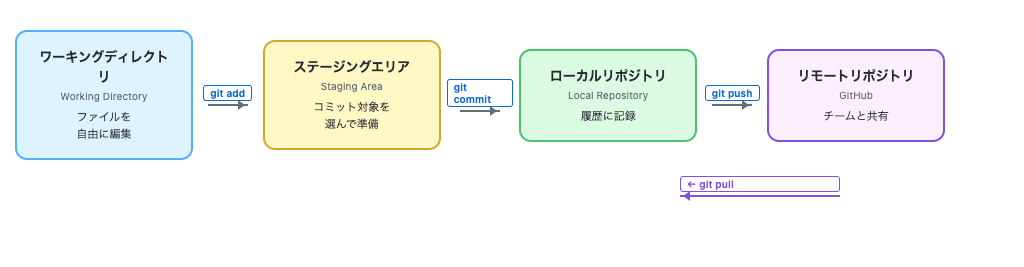
\includegraphics[width=0.9\textwidth]{images/diagram-4areas.png}
\end{figure}

\subsection{買い物にたとえて理解する}

この3つのエリアは、買い物のプロセスにたとえるとわかりやすくなります。

\textbf{ワーキングディレクトリ（Working Directory）} は、お店の中で商品棚を見ながら歩き回っている状態です。商品を手に取って見たり、棚に戻したりと、自由に行動できます。プロジェクトフォルダの中でファイルを編集している状態がこれに当たります。

\textbf{ステージングエリア（Staging Area）} は、「買い物カゴ」に相当します。棚から商品を選んでカゴに入れた状態です。まだ購入は確定していないので、カゴから商品を戻すこともできます。Gitでは \cmd{git add} でファイルをステージングエリアに追加します。インデックス（Index）とも呼ばれます。

\textbf{ローカルリポジトリ（Local Repository）} は、「レジで会計を済ませた」状態です。購入が確定し、レシート（コミット履歴）が発行されます。\cmd{git commit} でステージングエリアの内容が確定され、変更履歴として永続的に記録されます。

そして \textbf{リモートリポジトリ} は、「購入した商品を自宅に届ける」ようなものです。\cmd{git push} でローカルの履歴をGitHubに送信し、チームメンバーと共有します。

\subsection{なぜステージングエリアが必要なのか}

「編集したファイルを直接コミットすればいいのでは？」と思うかもしれません。しかし、ステージングエリアの存在には重要な意味があります。

たとえば、あなたが3つのファイルを編集したとします。そのうち2つはログイン機能の実装に関する変更で、残り1つはREADMEの誤字修正です。これらを1つのコミットにまとめてしまうと、後から履歴を見たときに「このコミットは何をしたのか」がわかりにくくなります。

ステージングエリアがあることで、「ログイン機能の変更だけを選んでコミット」→「READMEの修正を別のコミットとして記録」という、論理的に意味のある単位でコミットを作成できます。これは第6.5節のコミットメッセージの話とも密接に関わってきます。

\section{git status — 現在の状態を把握する}

\cmd{git status} は、Gitの作業中に最も頻繁に使うコマンドです。現在のリポジトリの状態 — どのファイルが変更されているか、どのファイルがステージングされているか、未追跡のファイルがあるか — を一目で把握できます。

\subsection{出力の読み方}

\cmd{git status} を実行すると、以下のような出力が表示されます。1つずつ意味を見ていきましょう。

\begin{lstlisting}[language=bash]
git status
\end{lstlisting}

\begin{lstlisting}[language={}]
On branch main
Your branch is up to date with 'origin/main'.

Changes to be committed:
  (use "git restore --staged <file>..." to unstage)
        modified:   README.md

Changes not staged for commit:
  (use "git add <file>..." to update what will be committed)
  (use "git restore <file>..." to discard changes in working directory)
        modified:   src/main.py

Untracked files:
  (use "git add <file>..." to include in what will be committed)
        new-file.txt
\end{lstlisting}

\textbf{1行目: \cmd{On branch main}} — 現在 \cmd{main} ブランチで作業していることを示しています。ブランチについては第7章で詳しく学びます。

\textbf{2行目: \cmd{Your branch is up to date with 'origin/main'.}} — ローカルの \cmd{main} ブランチがリモート（GitHub）の \cmd{main} ブランチと同じ状態であることを意味します。新しいコミットをプッシュしていない場合やリモートに新しいコミットがある場合は、別のメッセージが表示されます。

\textbf{\cmd{Changes to be committed:}（緑色で表示）} — ステージングエリアに追加されたファイルの一覧です。次に \cmd{git commit} を実行すると、ここに表示されているファイルの変更がコミットに含まれます。カッコ内には、ステージを取り消すためのコマンドが親切に表示されています。

\textbf{\cmd{Changes not staged for commit:}（赤色で表示）} — 変更されているがまだステージングされていないファイルです。\cmd{git add} でステージングするか、\cmd{git restore} で変更を元に戻すことができます。

\textbf{\cmd{Untracked files:}（赤色で表示）} — Gitが一度も追跡したことのない新しいファイルです。\cmd{git add} で追跡を開始できます。

\subsection{短縮表示}

頻繁に \cmd{git status} を実行する場合、短縮表示が便利です。

\begin{lstlisting}[language=bash]
git status -s
\end{lstlisting}

\begin{lstlisting}[language={}]
M  README.md       # 左側のMは「ステージ済みの変更」
 M src/main.py     # 右側のMは「未ステージの変更」
?? new-file.txt    # ??は「未追跡ファイル」
A  added-file.txt  # Aは「新規追加してステージ済み」
\end{lstlisting}

短縮表示では2列の文字で状態を表します。左列がステージングエリアの状態、右列がワーキングディレクトリの状態を示します。慣れると情報が一目で読み取れるようになります。

\section{git add — ステージングの操作と考え方}

\cmd{git add} は、ワーキングディレクトリの変更をステージングエリアに追加するコマンドです。「次のコミットに含めたい変更を選ぶ」操作と考えてください。

\subsection{基本的な使い方}

\begin{lstlisting}[language=bash]
# 特定のファイルをステージングする
git add README.md

# 複数のファイルを指定する
git add file1.py file2.py file3.py

# 特定のディレクトリ内の全ファイルをステージングする
git add src/

# カレントディレクトリ以下の全変更をステージングする
git add .

# リポジトリ全体の全変更をステージングする（削除されたファイルも含む）
git add -A
\end{lstlisting}

\subsection{なぜ全部addせず選ぶのか}

\cmd{git add .} や \cmd{git add -A} を使えばすべての変更を一度にステージングできます。しかし、先ほど説明したように、コミットは「論理的に意味のある単位」で作成することが望ましいのです。

たとえば、バグを修正している最中に、ついでにコードのインデントを整えたとします。このとき、バグ修正のファイルとインデント修正のファイルを別々のコミットにすることで、後から「バグ修正のコミットだけを取り消す」といった操作が可能になります。すべてを1つのコミットにまとめてしまうと、このような柔軟な対応ができなくなります。

\subsection{-pオプション：ファイルの一部だけをステージングする}

\cmd{git add -p}（\cmd{--patch}）は、1つのファイルの中から一部の変更だけをステージングできる強力なオプションです。

\begin{lstlisting}[language=bash]
git add -p src/main.py
\end{lstlisting}

このコマンドを実行すると、ファイル内の変更箇所が「ハンク（hunk）」という単位で1つずつ表示され、それぞれについて以下の選択肢が提示されます。

\begin{itemize}
  \item \cmd{y} — このハンクをステージングする
  \item \cmd{n} — このハンクをスキップする（ステージングしない）
  \item \cmd{s} — ハンクをさらに小さく分割する
  \item \cmd{q} — 終了する
\end{itemize}

この機能は、1つのファイルに複数の論理的に異なる変更を加えた場合に特に有用です。

\subsection{ステージングの取り消し}

間違えてステージングしてしまった場合は、\cmd{git restore --staged} で取り消すことができます。ステージングを取り消しても、ファイルの内容自体は変更されたままです。あくまでも「ステージングエリアから外す」だけの操作です。

\begin{lstlisting}[language=bash]
# 特定ファイルのステージングを取り消す
git restore --staged README.md

# すべてのステージングを取り消す
git restore --staged .
\end{lstlisting}

\section{git commit — 変更を記録する}

\cmd{git commit} は、ステージングエリアにある変更をローカルリポジトリに「確定」するコマンドです。コミットとは、プロジェクトのある時点の\textbf{スナップショット}（全体像の記録）に、メッセージや著者情報、タイムスタンプなどのメタデータを付けたものです。

\subsection{基本的な使い方}

\begin{lstlisting}[language=bash]
# メッセージを付けてコミットする
git commit -m "Add user authentication feature"

# 複数行のメッセージを書く場合
git commit -m "Add user authentication feature

- Implement login/logout endpoints
- Add password hashing with bcrypt
- Create user session management"

# エディタを開いてメッセージを書く場合（-m を省略する）
git commit

# 追跡済みファイルの変更をaddとcommitを同時に行う（新規ファイルは対象外）
git commit -am "Fix typo in README"
\end{lstlisting}

\cmd{git commit} を \cmd{-m} オプションなしで実行すると、第2章で設定したエディタ（VS Codeやvimなど）が開きます。長いコミットメッセージを書く場合や、フォーマットを丁寧に整えたい場合はこの方法が適しています。

\subsection{コミットメッセージの書き方の哲学}

コミットメッセージは、「未来の自分」や「チームメンバー」に向けた手紙のようなものです。3か月後にバグが見つかったとき、コミット履歴をたどって原因を探ることがあります。そのとき、\cmd{"fix"} や \cmd{"update"} としか書かれていないコミットが並んでいたら、原因調査は非常に困難になります。

良いコミットメッセージには、以下のルールがあります。

\textbf{構造のルール:}
\begin{itemize}
  \item \textbf{1行目（タイトル行）}: 50文字以内で変更の要約を書く。命令形（「Add...」「Fix...」「Update...」）で始める
  \item \textbf{2行目}: 空行にする（タイトルと本文を区切るため）
  \item \textbf{3行目以降（本文）}: 必要に応じて詳細な説明を書く。「なぜ」この変更が必要なのかを記述する
\end{itemize}

\begin{lstlisting}[language={}]
feat: Add dark mode support for the dashboard

The dashboard was difficult to use in low-light environments.
This commit adds a toggle switch in the header that switches
between light and dark themes using CSS custom properties.
\end{lstlisting}

\subsection{Conventional Commits}

チーム開発では、コミットメッセージの書き方を統一するために\textbf{Conventional Commits}という規約がよく使われます。これは、コミットメッセージの先頭に「タイプ」を示すプレフィックスを付ける方式です。

\begin{table}[htbp]
\centering
\begin{tabular}{llp{5cm}}
\hline
\textbf{プレフィックス} & \textbf{用途} & \textbf{例} \\
\hline
\cmd{feat:} & 新しい機能の追加 & \cmd{feat: Add dark mode support} \\
\cmd{fix:} & バグの修正 & \cmd{fix: Resolve login timeout issue} \\
\cmd{docs:} & ドキュメントのみの変更 & \cmd{docs: Update API reference} \\
\cmd{style:} & コードの意味に影響しない変更 & \cmd{style: Format with prettier} \\
\cmd{refactor:} & バグ修正でも機能追加でもない変更 & \cmd{refactor: Extract helper functions} \\
\cmd{test:} & テストの追加・修正 & \cmd{test: Add unit tests for auth} \\
\cmd{chore:} & ビルドプロセスやツールの変更 & \cmd{chore: Update dependencies} \\
\cmd{perf:} & パフォーマンスの改善 & \cmd{perf: Optimize database queries} \\
\cmd{ci:} & CI/CD設定の変更 & \cmd{ci: Add GitHub Actions workflow} \\
\hline
\end{tabular}
\end{table}

Conventional Commitsを採用すると、コミットの種類が一目で分かるだけでなく、コミット履歴から自動的にCHANGELOGを生成するツールとの連携も可能になります。

\begin{lstlisting}[language=bash]
# 良い例
git commit -m "fix: Prevent crash when user input is empty"
git commit -m "feat: Add CSV export for report page"
git commit -m "docs: Add contributing guidelines"

# 悪い例（何をしたかわからない）
git commit -m "fix"
git commit -m "update"
git commit -m "WIP"
git commit -m "asdfgh"
\end{lstlisting}

\subsection{--amend：直前のコミットを修正する}

コミットした直後に、タイプミスに気づいたり、ファイルを追加し忘れたりすることがあります。そのような場合に \cmd{--amend} オプションを使うと、直前のコミットを修正できます。

\begin{lstlisting}[language=bash]
# 直前のコミットメッセージだけを修正する
git commit --amend -m "fix: Correct the validation logic for email input"

# ファイルを追加し忘れた場合、追加してから amend する
git add forgotten-file.py
git commit --amend --no-edit   # --no-edit でメッセージはそのまま
\end{lstlisting}

\begin{quote}
\textbf{重要な注意}: \cmd{--amend} はコミットの内容を書き換えます。つまり、既にプッシュ済みのコミットを \cmd{--amend} で修正すると、ローカルとリモートの履歴が食い違い、トラブルの原因になります。\textbf{\cmd{--amend} はまだプッシュしていないコミットにのみ使う}、というルールを必ず守ってください。
\end{quote}

\section{git push — ローカルの記録をGitHubに送信する}

\cmd{git commit} で変更をローカルリポジトリに記録した後、その記録をGitHub（リモートリポジトリ）に送信するのが \cmd{git push} です。プッシュするまで、あなたのコミットは他のチームメンバーには見えません。

\subsection{基本的な使い方}

\begin{lstlisting}[language=bash]
# 基本のプッシュ（上流ブランチが設定済みの場合）
git push

# 初回プッシュ時（上流ブランチを設定する）
git push -u origin main
\end{lstlisting}

\subsection{-uオプション（--set-upstream）の意味}

初めてブランチをプッシュするとき、Gitは「ローカルのこのブランチは、リモートのどのブランチに対応するのか？」を知りません。\cmd{-u}（\cmd{--set-upstream}の省略形）オプションを付けることで、ローカルブランチとリモートブランチの対応関係（上流ブランチ、upstream branch）を設定します。

\begin{lstlisting}[language=bash]
# 初回: -u でローカルのmainとリモートのmainを関連付ける
git push -u origin main

# 2回目以降: -u は不要。git push だけでOK
git push
\end{lstlisting}

この設定は一度行えばリポジトリに記録されるため、同じブランチで2回目以降は \cmd{git push} だけで十分です。

\subsection{プッシュできない場合の対処}

チーム開発では、あなたが作業している間に他のメンバーがリモートにプッシュしていることがあります。この場合、あなたの \cmd{git push} は拒否されます。

\begin{lstlisting}[language=bash]
git push
# → ! [rejected]        main -> main (fetch first)
# → error: failed to push some refs to 'github.com:username/repo.git'
\end{lstlisting}

このエラーは「リモートにあなたが持っていない新しいコミットがあるので、まず取り込んでください」という意味です。対処方法は次のとおりです。

\begin{lstlisting}[language=bash]
# まずリモートの変更を取り込む
git pull

# コンフリクト（競合）が発生した場合は解決する（第8章で詳しく解説）

# その後、改めてプッシュする
git push
\end{lstlisting}

このように、Gitは「リモートの変更を無視して上書きする」ことを防ぐ安全機構を持っています。

\section{git pull — GitHubの変更をローカルに取り込む}

\cmd{git pull} は、リモートリポジトリ（GitHub）にある最新の変更をローカルに取り込むコマンドです。チーム開発では、作業を始める前に \cmd{git pull} を実行して最新の状態にするのが良い習慣です。

\subsection{基本的な使い方}

\begin{lstlisting}[language=bash]
# 基本のプル（上流ブランチから取り込む）
git pull

# 特定のリモート・ブランチを指定する
git pull origin main

# リベースモードでプルする（履歴がきれいになる）
git pull --rebase
\end{lstlisting}

\subsection{pull = fetch + merge}

\cmd{git pull} は実際には2つのコマンドを連続して実行しています。まず \cmd{git fetch} でリモートの最新情報をダウンロードし、次に \cmd{git merge} でダウンロードした変更をローカルブランチに統合します。

\begin{lstlisting}[language=bash]
# git pull は以下の2つのコマンドと同じ動作をする
git fetch           # リモートの最新情報をダウンロード（ローカルのファイルは変わらない）
git merge origin/main  # ダウンロードした変更をマージする
\end{lstlisting}

\subsection{fetchだけを使う理由}

\cmd{git fetch} を単独で使う場面もあります。\cmd{fetch} はリモートの情報をダウンロードするだけで、ローカルのファイルには一切手を加えません。これにより、「リモートでどのような変更があったのか」を安全に確認してから、マージするかどうかを判断できます。

\begin{lstlisting}[language=bash]
# リモートの最新情報を取得する（ローカルのファイルは変更されない）
git fetch

# リモートにある自分が持っていないコミットを確認する
git log HEAD..origin/main --oneline

# 内容を確認して問題なければマージする
git merge origin/main
\end{lstlisting}

この方法は、大きな変更がリモートにプッシュされている可能性があるとき、いきなりマージして自分の作業が壊れるのを避けたい場合に有用です。「まず偵察してから行動する」というアプローチです。

\section{git log — 履歴を確認する}

\cmd{git log} は、リポジトリのコミット履歴を表示するコマンドです。過去にどのような変更が、誰によって、いつ行われたのかを確認できます。

\subsection{基本的な使い方と各オプション}

\begin{lstlisting}[language=bash]
# 基本のログ表示（新しいコミットから順に表示される）
git log
\end{lstlisting}

基本の \cmd{git log} を実行すると、各コミットについてハッシュ値、著者、日時、コミットメッセージが表示されます。\cmd{q} キーを押すと表示を終了できます。

\begin{lstlisting}[language=bash]
# 1行表示（ハッシュの短縮形 + コミットメッセージだけを表示）
git log --oneline

# 出力例:
# a1b2c3d feat: Add dark mode support
# d4e5f6g fix: Resolve login timeout issue
# k0l1m2n Initial commit
\end{lstlisting}

\cmd{--oneline} はコミット全体を俯瞰するのに便利です。ハッシュ値は先頭7文字に短縮されますが、通常はこれでコミットを一意に特定できます。

\begin{lstlisting}[language=bash]
# グラフ表示（ブランチの分岐・合流を視覚的に表示）
git log --oneline --graph --all

# 出力例:
# * a1b2c3d (HEAD -> main, origin/main) feat: Add dark mode
# * d4e5f6g fix: Resolve login issue
# | * h7i8j9k (feature/api) feat: Add REST API
# |/
# * k0l1m2n Initial commit
\end{lstlisting}

\cmd{--graph} はブランチの分岐と合流をASCIIアートで描画します。\cmd{--all} はすべてのブランチを表示します（省略すると現在のブランチのみ）。

\begin{lstlisting}[language=bash]
# 最新の5件だけ表示する
git log -5

# 特定ファイルに関するコミットだけを表示する
git log -- README.md

# 変更内容（diff）も一緒に表示する
git log -p

# ファイルごとの変更行数の統計を表示する
git log --stat

# 特定の著者のコミットだけを表示する
git log --author="username"

# 日付で絞り込む
git log --since="2024-01-01" --until="2024-06-30"

# コミットメッセージにキーワードを含むものを検索する
git log --grep="fix"
\end{lstlisting}

\subsection{きれいなログ表示のエイリアス}

日常的に使うログ表示コマンドは長くなりがちです。Gitのエイリアス機能を使って、短いコマンドで呼び出せるように設定しておくと便利です。

\begin{lstlisting}[language=bash]
# エイリアスを設定する
git config --global alias.lg "log --oneline --graph --decorate --all"

# 設定後は以下のように使える
git lg
\end{lstlisting}

\cmd{--decorate} オプションは、ブランチ名やタグ名をコミットの横に表示します。先ほどの出力例で \cmd{(HEAD -> main, origin/main)} のように表示されていたのが、このオプションの効果です。

\section{git diff — 差分を確認する}

\cmd{git diff} は、ファイルの変更内容を詳細に確認するコマンドです。「何が変わったのか」を正確に把握するために使います。コミットやプッシュの前に差分を確認する習慣をつけると、意図しない変更を混入させるリスクを減らせます。

\subsection{4つの差分比較パターン}

\cmd{git diff} は、比較するエリアの組み合わせによって表示される内容が変わります。

\textbf{パターン1: ワーキングディレクトリとステージングエリアの差分（未ステージの変更）}

\begin{lstlisting}[language=bash]
git diff
\end{lstlisting}

まだ \cmd{git add} していない変更を表示します。最も基本的な使い方です。

\textbf{パターン2: ステージングエリアとリポジトリの差分（ステージ済みの変更）}

\begin{lstlisting}[language=bash]
git diff --staged
# または
git diff --cached   # --staged と同じ意味
\end{lstlisting}

\cmd{git add} してステージングしたが、まだコミットしていない変更を表示します。「次のコミットに含まれる内容」を確認するのに使います。

\textbf{パターン3: コミット間の差分}

\begin{lstlisting}[language=bash]
# 2つのコミット間の差分を表示する
git diff abc1234..def5678

# 直前のコミットと現在の差分
git diff HEAD~1..HEAD
\end{lstlisting}

特定のコミット間で何が変わったかを確認するときに使います。

\textbf{パターン4: ブランチ間の差分}

\begin{lstlisting}[language=bash]
# 2つのブランチの差分を表示する
git diff main..feature-branch
\end{lstlisting}

プルリクエストを作成する前に、mainブランチとの差分を確認するのに使えます。

\subsection{便利なオプション}

\begin{lstlisting}[language=bash]
# 特定ファイルの差分だけを表示する
git diff README.md

# 変更されたファイルの名前だけを一覧表示する（内容は表示しない）
git diff --name-only

# ファイルごとの変更行数の統計だけを表示する
git diff --stat

# 単語単位で差分を表示する（行全体ではなく変更箇所だけをハイライト）
git diff --word-diff
\end{lstlisting}

\cmd{--name-only} と \cmd{--stat} は、大量のファイルが変更されている場合に全体像を把握するのに便利です。まず \cmd{--stat} で概要を確認し、気になるファイルだけ \cmd{git diff ファイル名} で詳細を見る、という使い方がおすすめです。

\section{ファイルの移動・削除・変更取り消し}

日常の開発では、ファイルの名前を変えたり、不要になったファイルを削除したり、編集内容を元に戻したりすることがあります。これらの操作にもGit専用のコマンドがあります。

\subsection{ファイルの移動・名前変更（git mv）}

\begin{lstlisting}[language=bash]
# ファイル名を変更する
git mv old-name.py new-name.py

# ファイルを別のディレクトリに移動する
git mv src/utils.py lib/utils.py
\end{lstlisting}

\cmd{git mv} を使わず、OSのファイルマネージャやコマンド（\cmd{mv}）で名前を変えても動作しますが、Gitはそれを「旧ファイルの削除 + 新ファイルの追加」として認識します。\cmd{git mv} を使うと、Gitが「名前変更」として正しく追跡してくれます。

\subsection{ファイルの削除（git rm）}

\begin{lstlisting}[language=bash]
# Gitの追跡からもディスクからも削除する
git rm unnecessary-file.py

# Gitの追跡だけ解除し、ディスク上にはファイルを残す
git rm --cached secret.env
\end{lstlisting}

\cmd{git rm --cached} は、第5章の \cmd{.gitignore} の節で解説した「既に追跡されたファイルを無視する」場面で特に重要です。

\subsection{変更の取り消し}

ファイルを編集したが、やっぱり元に戻したい、という場面は頻繁にあります。\cmd{git restore} コマンドで元に戻すことができます。

\begin{lstlisting}[language=bash]
# ファイルの変更を元に戻す（ワーキングディレクトリの変更を取り消す）
git restore README.md

# 全ファイルの変更を元に戻す
git restore .

# ステージングを取り消す（変更自体はワーキングディレクトリに残る）
git restore --staged README.md
\end{lstlisting}

\begin{quote}
\textbf{注意}: \cmd{git restore} で元に戻した変更は、コミットされていない限り復元できません。本当に不要な変更かどうかを確認してから実行してください。
\end{quote}

\section{実践：一連の開発フローを体験する}

ここまで学んだコマンドを使って、実際の開発フローを一通り体験してみましょう。新しいリポジトリを作成するところから、ファイルを編集してコミット・プッシュするまでの流れをステップバイステップで進めます。

\begin{lstlisting}[language=bash]
# ステップ1: リポジトリをクローンする
git clone git@github.com:username/my-project.git
cd my-project

# ステップ2: 現在の状態を確認する
git status
# → "nothing to commit, working tree clean" と表示されるはず

# ステップ3: 新しいブランチを作成して切り替える（詳しくは第7章）
git switch -c feature/add-login

# ステップ4: ファイルを編集する（エディタで自由に作業）
# ここでは src/auth.py を新規作成したとします

# ステップ5: 状態を確認する
git status
# → Untracked files: に src/auth.py が表示される

# ステップ6: 差分を確認する（新規ファイルの場合は内容全体が差分として表示）
git diff

# ステップ7: ファイルをステージングする
git add src/auth.py

# ステップ8: ステージングされた内容を確認する
git diff --staged

# ステップ9: コミットする
git commit -m "feat: Add login functionality"

# ステップ10: さらに作業を続けてコミットする
# ... テンプレートファイルを編集 ...
git add src/templates/login.html
git commit -m "feat: Add login page template"

# ステップ11: 履歴を確認する
git log --oneline
# → 2つのコミットが表示される

# ステップ12: GitHubにプッシュする
git push -u origin feature/add-login

# ステップ13: GitHubでプルリクエストを作成する（第10章で詳しく解説）
gh pr create --title "feat: Add login feature" --body "Login機能を追加"
\end{lstlisting}

この流れが、日常的な開発作業の基本パターンです。慣れてくると、\cmd{status} → \cmd{add} → \cmd{commit} → \cmd{push} のサイクルが自然に身についてきます。最初のうちは、各ステップの間に \cmd{git status} を挟んで状態を確認する習慣をつけると、Gitの動作への理解が深まります。

\section{まとめ}

この章では、Gitの日常的なワークフローの中核となるコマンド群を学びました。

\begin{itemize}
  \item \textbf{3つのエリア}: ワーキングディレクトリ → ステージングエリア → ローカルリポジトリという3段階の構造が、Gitの柔軟性の源泉である
  \item \textbf{git status}: 作業中に最も頻繁に使うコマンド。現在の状態を把握する習慣をつけよう
  \item \textbf{git add}: コミットに含める変更を選択する。\cmd{-p} オプションでファイル内の一部だけをステージングすることもできる
  \item \textbf{git commit}: 変更を履歴に確定する。コミットメッセージは「未来の自分への手紙」として丁寧に書こう。Conventional Commitsの規約が広く使われている
  \item \textbf{git push}: ローカルの記録をGitHubに送信する。初回は \cmd{-u} で上流ブランチを設定する
  \item \textbf{git pull}: GitHubの変更を取り込む。内部的にはfetch + mergeの2段階で動作する。安全を期すなら \cmd{fetch} だけで偵察してからマージするとよい
  \item \textbf{git log}: 履歴を確認する。\cmd{--oneline --graph --all} の組み合わせが特に便利
  \item \textbf{git diff}: 差分を確認する。ステージ前・ステージ後・コミット間・ブランチ間の4パターンを使い分ける
\end{itemize}

次の章では、チーム開発に不可欠な「ブランチ」の概念と操作を学びます。ブランチを使いこなすことで、複数の機能を同時に、安全に開発できるようになります。
